\documentclass[../lab2.tex]{subfiles}

\begin{document}

    \begin{figure}[!htb]
        \begin{minipage}{0.48\textwidth}
            \centering
            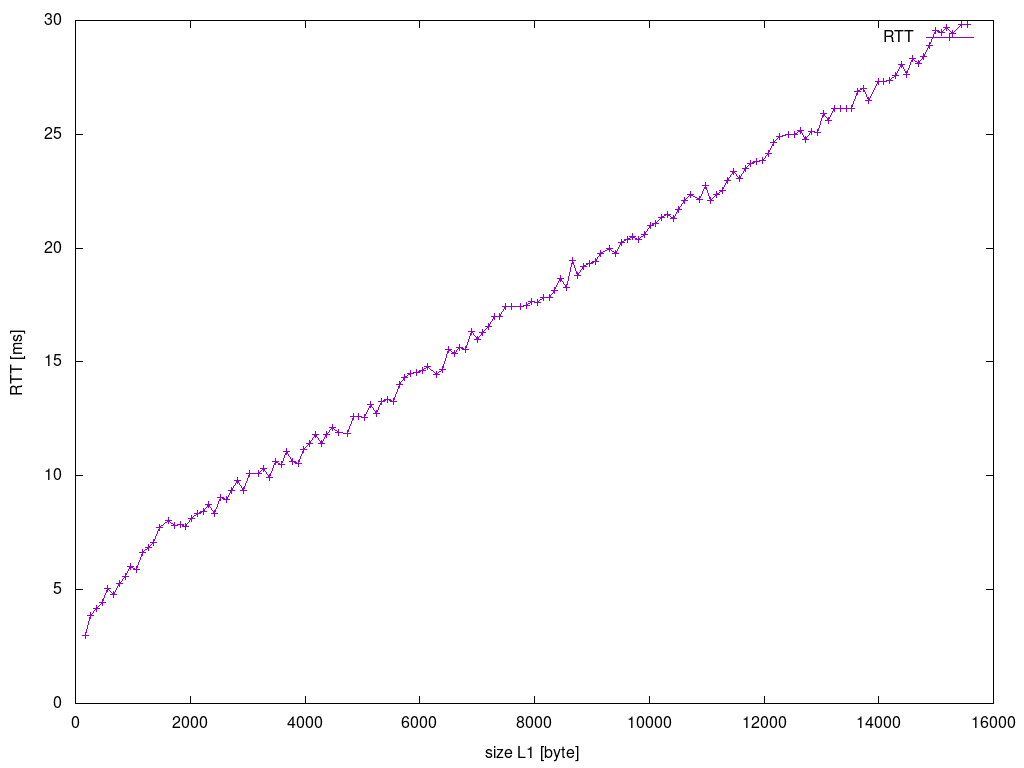
\includegraphics[width=1\linewidth]{RTTW.png}
            \vspace{-20pt}
            \caption{RTT}\label{RTTW}
        \end{minipage}\hfill
        \begin{minipage}{0.48\textwidth}
            \centering
            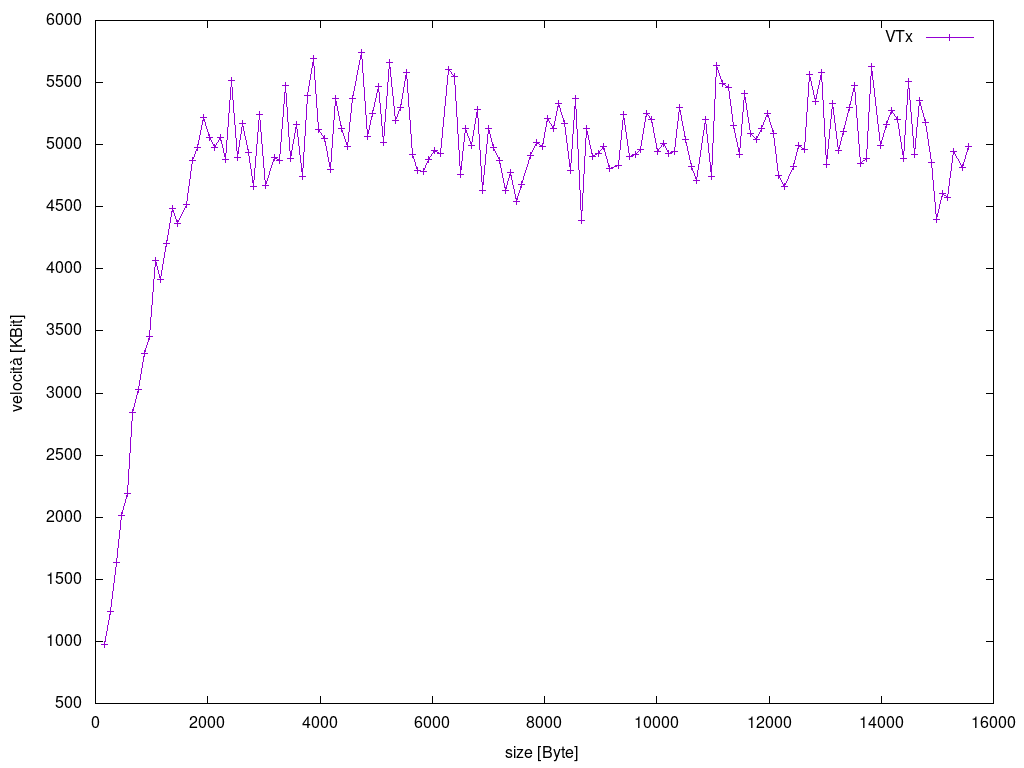
\includegraphics[width=1\linewidth]{VTxW.png}
            \vspace{-20pt}
            \caption{VTx}\label{VTxW}
        \end{minipage}
    \end{figure}

    Avendo impostato la velocità di connessione tra Pc Live Linux e router a 10Mb/s
    l'unica incognita rimane la velocità della connessione wireless.
    Ipotizzando il caso in cui $V_{TX1} < V_{TX2}$, indicando con $V_{TX1}$ la velocità della connessione wireless 
    e con $V_{TX2}$ la velocità tra Pc Live Linux e Router,e' possibile ricavare:

    \begin{equation}
        \centering
        \begin{cases}
            RTT = \frac{2D}{V_{TX2}} +\frac{2D}{V_{TX1}} + T_\eta  \qquad \, \, \, D < 1500 \\
            \\
            RTT = \frac{2D}{V_{TX2}} +\frac{2MTU}{V_{TX1}} + T_\eta  \qquad D > 1500
        \end{cases}
    \end{equation}

    \begin{equation}
        \centering
        V_{TX1} = \frac{2D}{RTT - \frac{2MTU}{V_{TX2}}} 
    \end{equation}
    
    \vspace{10pt}

    Abbiamo riportato l'andamento della velocità del WiFi approssimando l'\textit{header} WiFi a
    40 Byte. \\
    Come si può notare analogamente ai punti precedenti all'aumentare della dimensione
    del pacchetto si arriva a una stima più accurata della velocità poiché si possono 
    trascurare con meno margine di errore i tempi di propagazione e elaborazione, 
    cioe' il fattore $T_\eta$.
    Dall'andamento del grafico si può notare un comportamento poco
    regolare, probabilmente dovuto alla minore affidabilità del mezzo trasmissivo 
    e ad una maggiore sensibilità al rumore dovuto a fonti esterne, 
    rispetto ad un cavo fisico.

\end{document}